\chapter{State of the art}
\label{chapter:research}

\section{Technologies}
\subsection{Python}

Python \cite{python} is a multi-paradigm high-level programming language whose design philosophy emphasizes code readability. It allows programmers to write clear programs faster and easier than it would be possible in other languages such as C.

We have chosen python as our language due to a number of reasons. Firstly, some of the tools that we will use are written in python. While it would have been possible to write the rest of the project in a different language, it would have introduced communication bottlenecks and performance issues. EVE Online is also developed using python, so there’s a close correlation between the game itself, the databases and our toolset. 

Another selling point was the community of developers behind the language. There are a plethora of modules written for python ranging from archive managers, all the way to scientifical frameworks. Taking advantage of them will prove much easier than having to write new libraries ourselves.

Moreover, from a programming perspective, python provides functionalities like list comprehension and elements of functional programming that make it easy to write an engine that works with expression trees and lists of heterogeneous entities. There is also Django, a framework that makes writing web apps a total breeze.

In the end, python was a clear choice because it’s a powerful language that suited our design philosophy and has a great community to support the developers.

However, while writing our engine in pure C might prove very difficult, the performance boost might outweigh the effort. In the future we will look on porting it to C and maybe even Javascript to allow client-only fitting tools.

\subsection{MySQL}
MySQL \cite{mysql} \cite{mysqlhigh} is one of the best-known relational database management systems \footnote{http://en.wikipedia.org/wiki/Relational_database_management_system} out there. It is a popular choice of database for use in web applications and a central component of the widely used LAMP \footnote{http://en.wikipedia.org/wiki/LAMP_(software_bundle)} open source web application software stack.

MySQL has support for independent storage engines like MyISAM for read speed, InnoDB for transactions and referential integrity and MySQL Archive for storing historical data in little space. MyISAM also supports full text indexing and searching which proves highly valuable when performing keyword searches.

Early development of the project used MySQL as the database backend because of its high performance and ease of deployment. However, due to the fact that the python binding hasn’t yet been ported to python 3, we were forced to switch to SQLite, which has a proper python 3 implementation.

\subsection{SQLite}
SQLite \cite{sqlite} is a popular database backend, favored by many due to its simplicity and performance. Unlike other backends, SQLite maintains all information in a single file. This makes migration an extremely easy process since there are no servers that have to be configured and restarted. All you have to do is copy the database file and point your frameworks to it.

It implements this simple design by locking the entire database file during writing. SQLite read operations can be multitasked, though writes can only be performed sequentially. This makes for great performance when reading the database, but writing to it can be very slow. Moreover, INSERT operations are issued in a transaction, making them even slower as the transaction overhead can be far greater than the operation itself.

Using python 3 restricted us to use SQLite, which in the long run proved favorable due to the ease of migration. While performance suffered a bit, we might stick with this backend as CCP will soon provide sqlite dumps of their database.

\subsection{Javascript}
Javascript \cite{javascript} is a highly versatile interpreted language used to power today’s dynamic websites. Through it, websites can interact with the user, control the browser, communicate asynchronously and alter document content. Recently, it has gained popularity in game development, as well as in desktop applications.

Javascript is a prototype based scripting language with a syntax influenced by C and key design principles borrowed from Scheme. Like Python, it is a multi-paradigm language, supporting object-oriented, imperative and functional programming styles.

The UI of the project is written entirely in Javascript using libraries like jQuery \cite{jquery} and jQuery UI \cite{jqueryui} which enabled us to provide cross-platform features that don’t require any extra plugins to work.

\subsection{Django}
One of the most well-known python packages, Django \cite{django} is a framework for building web applications in python that comes with its own Object Relational Mapping \footnote{https://en.wikipedia.org/wiki/Object-relational_mapping} framework, along with a caching framework, internationalization support and a template engine.

The template engine allows a clear separation between code and design. The framework supports template files in which one writes the design part of the application. These templates are then fed with data coming from the application which is inserted in the templates through the use of tags.

One big advantage of having the design and code separated is that you can have separate programmers maintain each of them. Web developers can handle the application logic while web designers can produce the layout.

With its multitude of frameworks, Django allowed us to focus on code rather than deal with how to build a web platform. This made it possible to start writing code on day 1 without having to worry about implementing proper session management.

\subsection{jQuery}
jQuery \cite{jquery} is a cross-browser Javascript library designed to simplify client-side scripting. It makes it easier to navigate a document, manipulate the DOM\footnote{Document Object Model} tree, create animations, handle events and develop Ajax applications. It also takes on a modular approach, developers being able to easily write plugins that can take advantage of the library’s power.

The UI uses jQuery to provide users with a sleek interface that is easy to navigate and understand, but rich in features to satisfy any hardcore user. All DOM manipulations are handled through the library, while certain plugins are used to implement features like persistence through cookies, sortable lists and draggable elements.

\subsection{HTML5}
HTML5 \cite{html5} is the fifth revision of the HTML standard that aims to improve the language with support for the latest multimedia while keeping it easily readable by humans and consistently understood by computers and devices. It extends and improves the markup available for documents and introduces APIs for complex web applications.

We make use of HTML5 through the new data attributes \cite{html5data} that allow arbitrary data to be stored for any element. This allows state information to be attached to their containers which can be retrieved easily without having to keep it separate in Javascript objects. Another useful feature of HTML5 is the ability to change the current URL without a page refresh. We do this every time a user browses fits so he/she can easily copy and share the link for it without having to use a separate form.

\subsection{CSS3}
Cascading Style Sheets \cite{css} is a style sheet language used for describing the presentation semantics (the look and formatting) of a document written in a markup language. CSS is designed to separate content from presentation (layout, colors, fonts etc.).

The UI has builtin support for themes which can change the look and feel of the interface. These themes consist of a collection of CSS files which style different parts of the UI.

Some notable CSS3 features that are used in the UI are animations \cite{cssanimations} and box sizing \cite{cssboxsizing}. Animations allow transitions between two states, while box sizing sets how size calculations are performed in the box layout.

\section{Research}
\subsection{Items database}
\begin{figure}[h]
\centering
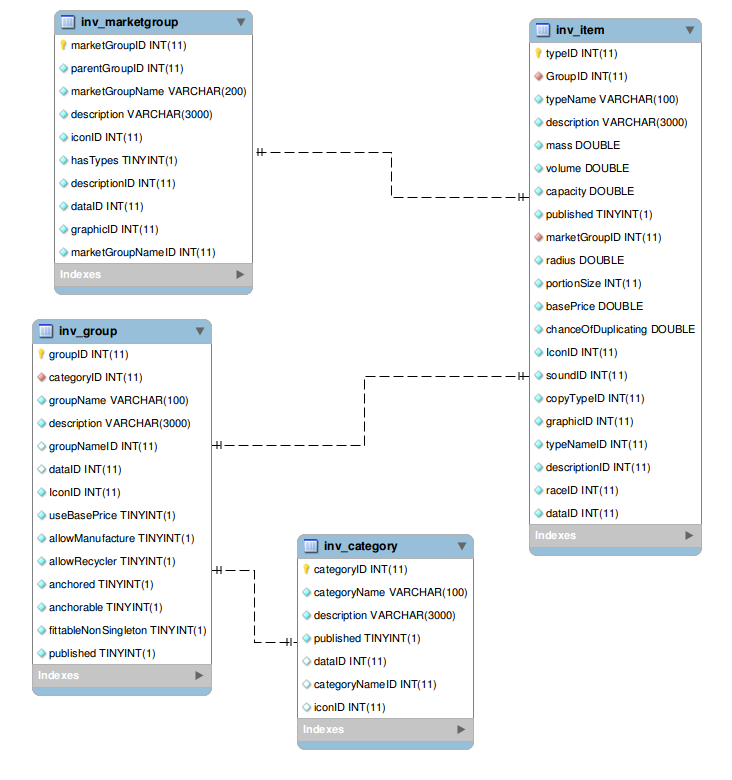
\includegraphics[width=0.7\linewidth]{src/img/items}
\caption{Types and groups}
\label{fig:items}
\end{figure}

As you can see in diagram \ref{fig:items}, all inventory types (including ships, modules and skills) are stored in a table called inv_item. Every item has a unique identifier called typeID. Also, each item belongs to a market group as illustrated by the foreign key marketGroupID. Market groups are the ones that appear in the market browser. They can be nested, while the leaf groups have the column hasTypes set to True, which indicates that the respective market group is the holder for the items.

Besides market groups, items also have a separate inventory group, as shown by the foreign key groupID. These groups do not show in the game and they don’t have a 1-to-1 correspondence with the market groups. They are more abstract groups and often, items that would fall under multiple market groups, reside in a single inventory group.

Inventory groups have associated an inventory category using the foreign key categoryID. These are top level abstract categories that contain many items. For instance, any ship, regardless of its market group, falls under the Ship category. The same goes for modules which reside in the Modules category. These categories can be used in JOINs to easily fetch all ships or all items in the market. This functionality will prove very helpful when performing item or ship searches.

Some simple attributes, like mass and volume, reside in the inventory items table. The rest of the attributes are found in the dogma attributes table, illustrated in diagram \ref{fig:dogmaattribs}.

\begin{figure}[h]
\centering
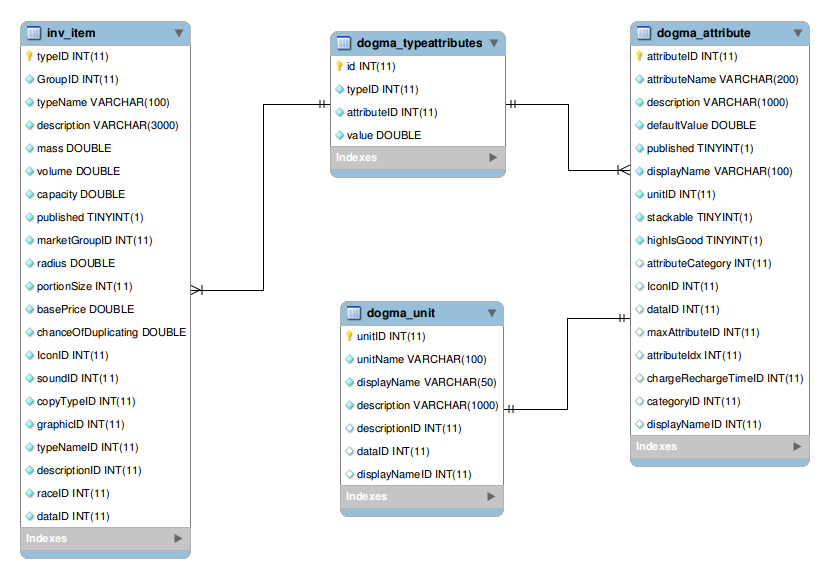
\includegraphics[width=0.7\linewidth]{src/img/dogmaattribs}
\caption{Dogma attributes}
\label{fig:dogmaattribs}
\end{figure}

Each attribute has an attributeID and an attributeName used for identification. The displayName column is the name that is shown ingame. The foreign key unitID points to the dogma unit table that contains measurement units such as kilogram for mass and second for time. The stackable column specifies whether that attribute has a stacking penalty \cite{stacking} that applies when more than one module that affects the same attribute are fitted on a ship. More on that in the Dogma section.

The dogma type attributes table specifies many-to-many relations between inventory items and their attributes. Each association has a value column that represents the value of that attribute for that module. There are many weird attributes present in the table for historical or unknown reasons. On the other hand, some are missing. For instance, the warpSpeedMultiplier attribute specifies how many times faster the ship’s warp speed is compared to the baseWarpSpeed attribute, which is not present in the table, but rather hardcoded to the value 3.

Another oddity is that, while present, the attribute for cargo capacity is never set on any of the ships. Instead, this attribute is set in the items table. Not following this rule is the attribute for the ship’s mass, which is set both in the items table and in the attributes table.

CCP’s codebase has been constantly evolving so it’s quite common to find such inconsistencies. The database also hosts a lot of internal testing data or data restricted to game masters and administrators. This data usually has the published column set to False, so a quick filtering by that column will only return the items that are actually present in the game.

\subsection{Dogma}
The items and attributes table are enough to learn about the modules in the game, but to see how they function we need to look into dogma effects and expressions.

\begin{figure}[h]
\centering
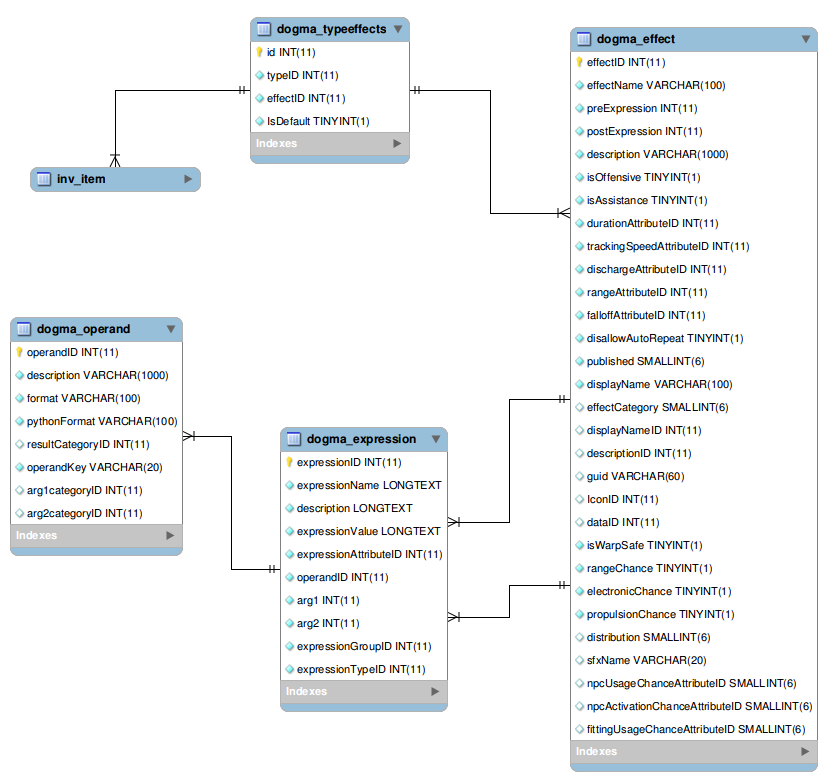
\includegraphics[width=0.7\linewidth]{src/img/dogma}
\caption{Dogma effects and expressions}
\label{fig:dogma}
\end{figure}

Every item present in the items table has at least one dogma effect attached to it through the dogma type effects table. These effects describe what the item does and how it affects the ship, the character flying the ship and the enemy being targeted by the ship.

The main parts of a dogma effect are the preExpression and postExpression attributes, that both link to a dogma expression. The preExpression specifies what the module does when it becomes active, while the postExpression specifies what happens when the module becomes inactive. The active/inactive state can mean different things for different modules.

Passive modules become active once they are fitted to the ship and onlined. They become inactive when they are offlined or removed from the ship. In the case of active modules, the pre and post expressions refer to the start and end of the module’s cycle. For instance, shield rechargers apply their bonus to the ship’s shields at the start of the cycle. In this case, the preExpression will specify that, at the start of the cycle, the module will consume capacitor and boost the ship’s shield. At the end of the cycle, the module will do nothing. Armor repairers apply their bonus at the end of the cycle. The preExpression in this case will include the effect for consuming capacitor, while the postExpression will apply the repairing bonus.

It is important to differentiate between these two types of behaviour as simulators can only be accurate if the effects are applied at the right time and in the right circumstances.

A dogma expression consists of a left and right argument that are actually expressions themselves and an operand that is applied to the two arguments. There are a number of special expressions that will actually point to the ship or character entity so that they can be used as part of much larger expressions. These expressions do not have the second argument set to anything.

When an expression needs to refer to an attribute, it sets the operandID to 22 (defAttr) and the attributeID value to the actual id of the attribute. It also ignores the arg1 and arg2 values. If the targeted attribute is stackable, then the effect receives a stacking penalty which is calculated depending on the number of modules affecting it. Thus, if only one module affects an attribute, then it will apply 100\% of its bonus. If a second module is fitted that targets the same attribute, then it will only apply its bonus with an 87\% efficiency. This efficiency drops exponentially with the number of modules. The following formula is used to calculate the penalty:

\begin{equation}
S(n) = 0.5^{\left(\frac{n-1}{2.22292081}\right )^{2}}
\end{equation}

Now let’s look at a couple of dogma expressions.

\begin{lstlisting}[label=dogma_expr1, caption=An example of a dogma expression]
(SkillCheck(OnlineHasSkillPrerequisites)) AND (If(CurrentShip.cpuOutput()>=(CurrentShip.cpuLoad())+(CurrentSelf.cpu())), Then (If(CurrentShip.powerOutput()>=(CurrentShip.powerLoad())+(CurrentSelf.power())), Then (CurrentSelf->isOnline := Int(1));     (((CurrentShip->cpuLoad).(ModAdd)).AddItemModifier (cpu));     (((CurrentShip->powerLoad).(ModAdd)).AddItemModifier (power)) OR UserError(NotEnoughPower)) OR UserError(NotEnoughCpu))
\end{lstlisting}

The above effect tells us a number of things. First, it checks whether the character has the proper skills needed to use the module. Then, it checks whether the ship has enough CPU and Power to fit the module. If these conditions are met, then the module is onlined and the CPU and Power levels are updated to reflect the newly fitted item. If the ship cannot sustain the module, then an error is thrown.

\begin{lstlisting}[caption=Another example of a dogma expression]
((CurrentShip->shieldCapacity).(ModAdd)).AddItemModifier (capacityBonus)
\end{lstlisting}

The above effect tells us that the capacityBonus attribute is being added to the current ship’s shield capacity.

\subsection{Capacitor}
The capacitor is the ship’s main power supply that acts like a rechargeable battery. As modules are activated, power is drained from the capacitor, which then starts to recharge. A capacitor has two attributes: capacity (how much power it can store) and recharge time (how much time is needed for the reactor to fill it).

\subsubsection{Capacity}
The amount of power that capacitors can store varies, although usually it varies by size of ship: the larger the ship, the larger the capacitor. The capacity can be increased directly by training the Energy Management \footnote{http://wiki.eveonline.com/en/wiki/Energy_Management} skill. Also, a huge variety of skills, and in particular those in the Engineering \footnote{http://wiki.eveonline.com/en/wiki/Item_Database:Skills:Engineering} tree, reduce the amount of power needed to activate modules, thus indirectly improving capacity. The capacity can be further increased using specialized modules, such as capacitor batteries \footnote{http://wiki.eveonline.com/en/wiki/Item_Database:Ship_Equipment:Engineering_Equipment:Capacitor_Batteries}, power diagnostic systems \footnote{http://wiki.eveonline.com/en/wiki/Power_Diagnostic_System_I} and rigs \footnote{http://wiki.eveonline.com/en/wiki/Large_Capacitor_Control_Circuit_I}.

\subsubsection{Recharge time}
The amount of time to fully recharge a capacitor also varies, in this case usually by the size of the capacitor: smaller capacitors tend to recharge faster. Capacitor recharge time can be reduced directly by training certain skills or fitting certain items such as cap rechargers \footnote{http://wiki.eveonline.com/en/wiki/Cap_Recharger_I} and flux coils. 

\subsubsection{Role in combat}
If the capacitor becomes fully drained, a ship may be unable to fire its weapons, warp out from combat, or use any of its modules, and may wind up being left with only the ability to launch drones and move around. Running out of capacitor power in the middle of combat can be fatal.

There are modules that can neutralize an opponent's capacitor power, steal it and add it to your own, or allow allies to transfer it among each other. Therefore capacitor management is a notable aspect in warfare. 

\subsubsection{Role in navigation}
Capacitor is also used by the ship's warp drive. The longer the distance is, the more energy is needed to initiate the warp. Sometimes a ship cannot make a very long warp in a single try, thus requiring to make more than one warp and allow the capacitor to recharge between them. 

\subsection{Recharge rate}
Many EVE pilots have tried to determine the precise formula for the capacitor recharge rate --- the speed at which the ship's capacitor refills itself with energy. Through observation of various experiments, it has been concluded that the recharge rate is not a linear function, but has a more complex shape, as can be seen in Figure \ref{fig:ratevstime}.

By taking various ships and fully depleting their capacitor, we could observe how it recharges to full capacity. Experiments have shown that peak recharge rate is at near 20\% of the capacitor’s recharge time, as illustrated by Figure \ref{fig:ratevstime}.

\begin{figure}[h]
\centering
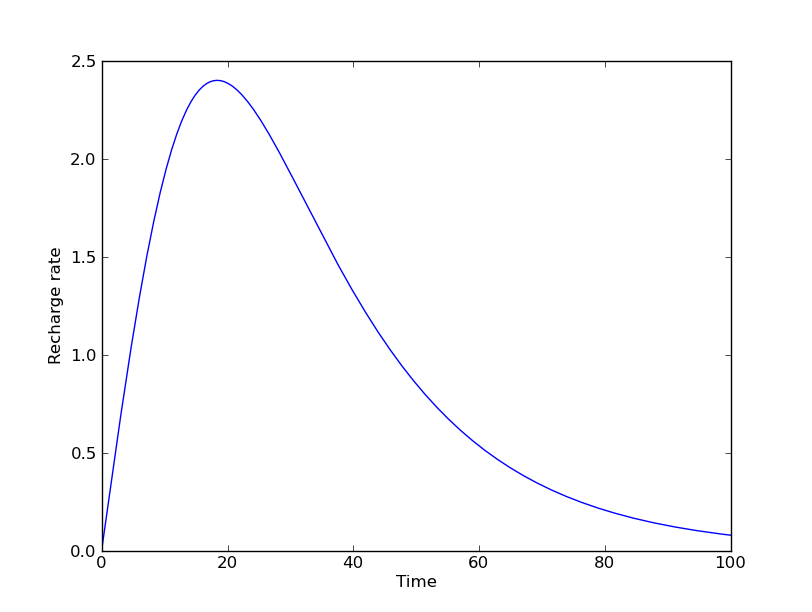
\includegraphics[width=0.7\linewidth]{src/img/ratevstime}
\caption{Capacitor recharge rate evolution over time}
\label{fig:ratevstime}
\end{figure}

Research \cite{capresearch} done by various members of the community has shown that the actual formula for recharge rate is:

\begin{equation}
C = C_{MAX} * \left(1-\frac{1}{\cosh (\tau * t)}\right)
\label{eq1}
\end{equation}

Where:
\begin{itemize}
\item $ C_{MAX} $ is the maximum charge of the capacitor.
\item $ \tau $ is a time constant equal to $ \frac{k}{T} $, where T is the recharge time.
\end{itemize}

It has been shown that k is approximately 4.8 \cite{capresearch}.

Taking the derivative of Equation \ref{eq1}, we get the formula for instantaneous cap recharge rate:

\begin{equation}
\frac{dC}{dt} = C_{MAX} * \tau * \frac{\tanh (\tau * t)}{\cosh (\tau * t)}
\label{eq2}
\end{equation}

We isolate t from Equation 1 and obtain:
\begin{equation}
t = \frac{1}{\tau} * acosh \left(\frac{1}{1 - \frac{C}{C_{MAX}}}\right)
\label{eq3}
\end{equation}

\begin{equation}
\tanh \left(acosh \left(\frac{1}{1 - \frac{C}{C_{MAX}}}\right) \right) = \sqrt{2 * \frac{C}{C_{MAX}} - \left(\frac{C}{C_{MAX}}\right) ^ 2}
\label{eq4}
\end{equation}

Using equations \ref{eq1}, \ref{eq3} and \ref{eq4} we obtain:

\begin{equation}
R(C) = C_{MAX} * \tau * \left(1 - \frac{C}{C_{MAX}}\right) * \sqrt{2 * \frac{C}{C_{MAX}} - \left(\frac{C}{C_{MAX}}\right) ^ 2}
\end{equation}

\begin{figure}[h]
\centering
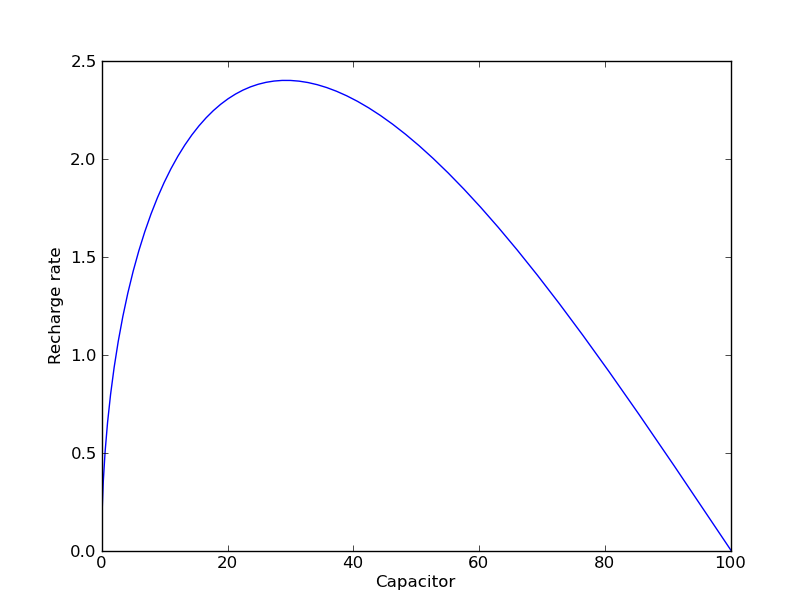
\includegraphics[width=0.7\linewidth]{src/img/ratevscap}
\caption{Capacitor recharge rate vs capacitor state}
\label{fig:ratevscap}
\end{figure}


The local maximum for Equation \ref{eq2} occurs at $ t \cong 18.3619 $, which corresponds with the inflection point for Equation \ref{eq1}. This means that, at 18\% of the recharge time, the recharge rate is at its peak. However, this does not mean that the capacitor is at 18\% of its max charge. To find that, we substitute $ t = 0.18 * T $ in Equation \ref{eq1} and get $ C = 0.284 * C_{MAX} $. So the capacitor recharges fastest at approximately 28\% of its max charge. These numbers are backed up by real life observations.

\begin{figure}[h]
\centering
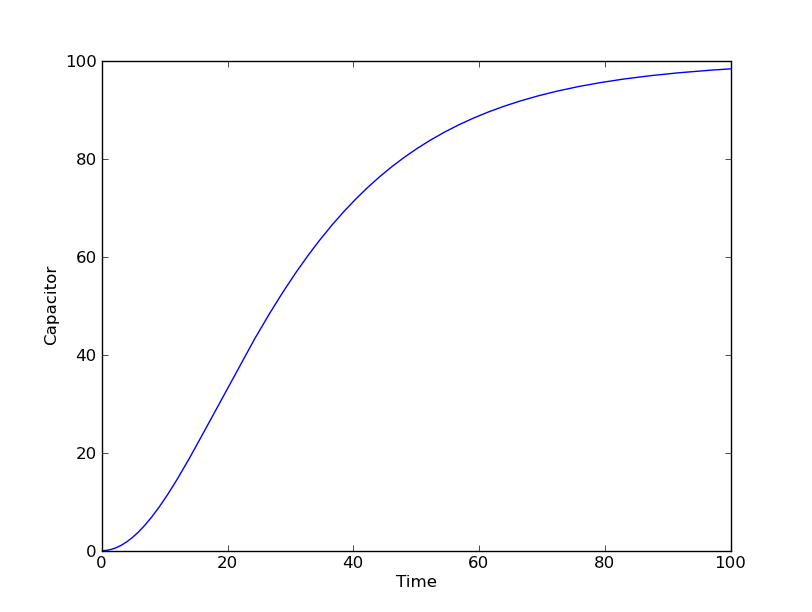
\includegraphics[width=0.7\linewidth]{src/img/capvstime}
\caption{Capacitor evolution over time}
\label{fig:capvstime}
\end{figure}


\subsection{Capacitor stability}
Players are interested in the point where the capacitor is stable - at which you can sustain all your active modules and not run out of cap. That situation is commonly referred to be cap stable.

This is an important metric for any ship because it provides invaluable information in combat: how much you can last before having your capacitor fully drained, how much you can keep certain modules active or how and when you should activate certain cap hungry modules.

In order to find this point, one must look at the recharge rate function graph illustrated above. If you think of the combined drain of all active modules as a straight line on that graph, parallel to the OX axis\footnote{All modules will drain the same amount of cap, regardless of the state of the capacitor.}, then there’s 3 possible situations:

\begin{itemize}
\item The drain is larger than the peak recharge rate, illustrated by the line being above the curve. In this scenario the capacitor won’t be able to sustain the active modules and will fully deplete. The metric in this case is the amount of time till full depletion.
\item The drain is equal to the peak recharge rate, illustrated by the line being tangent to the curve. In that case, the capacitor will drop to the point determined by the peak value and then be able to sustain all the active modules. The metric in this case would be that single point.
\item The drain is lower than the the peak recharge rate. In that case, there will be two cap stable points (illustrated by the line intersecting the curve in 2 points) at which the capacitor can sustain all active modules. The library will return both points, leaving it up to the next layer to decide which to display.
\end{itemize}

There are two approaches to finding these points. One would be to assume that the activation cost of an active module is drained over time, thus calculating an average per second of cap drained. All these averages could be added up and divided by the number of active modules, thus ending up with a total average of cap drained per second. This model would result in a straight line represented on the recharge graph that would yield 1 or 2 cap stable points. This approach would be very computationally light weight, but provide a rather inaccurate measurement.

The other, more CPU intensive method, would be to consider the activation costs as instantaneous bursts of cap drain (which is a correct assumption) and simulate the drain over time in small steps. You start with a full capacitor and at t = 0 all modules are activated resulting in a spike of cap drain as every module bites a portion of the capacitor. A period of time passes in which the capacitor has time to recharge until the module with the shortest cycle activates again. More such intervals pass in which the capacitor tries to sustain the active drain. At a moment in time, determined by the smallest common multiple of the module cycles, all modules will again simultaneously activate resulting in another huge spike. The interval between two such spikes shall be referred to as a drain period.

There can be more than one drain period until the capacitor reaches a cap stable point, or, in case the drain is too much, fully deplete. The simulator will run until the cap level stabilizes around a point - the first stability point. By equating the recharge rate function with the value of it in that point, we obtain the second stability point.

\subsection{Effective Hit Points and Resistances}
While there are so many different ways of sustaining damage, there is one metric that applies to the majority of them and that is the number of Effective Hit Points. This number represents the total incoming damage the ship can sustain until it explodes. It only makes sense when it is associated with an incoming damage pattern.

There are 4 types of resistances than can be applied to shield, armor and hull. These are Electromagnetic, Thermal, Kinetic and Explosive. Each of them signifies how well the ship absorbs incoming damage of that type. For instance, if the shields of a ship have 50\% Kinetic resistance, that means that any enemy shooting the ship with Kinetic ammo will only do 50\% of its damage. In the database, these attributes are called resonances\footnote{Resonance = 1 - Resistance} and they’re actually incoming damage multipliers. So a 0\% resistance translates to a 100\% resonance.

EHP is calculated by multiplying the base hit points of shields, armor and hull with $ \frac{1}{resonance[type]} $. If a ship has 50\% Kinetic resistance for shields, 1000 shield hitpoints and the enemy is shooting Kinetic ammo, then that ship will have 2000 effective shield hitpoints.

\subsection{Shields}
A ship’s shields are the only kind of defense that regenerates over time. The recharge rate is the same as the capacitor’s so the same module used to simulate capacitor drain can be used to simulate incoming damage. The key difference would be that some modules, instead of draining the shields, would add to it. This would not require any change in the simulator since these modules would just have a negative drain.

\subsection{Damage per second}
A ship’s main metric for damage output is the amount of damage per second (DPS). Every type of gun hits for a certain amount of damage called alpha damage every cycle. By dividing alpha damage by the cycle time you get the amount of DPS that weapon can output. Adding them all up gives the ship’s DPS. This can consist of turrets and missiles damage, drone damage and smartbomb damage.

There are two ways of calculating DPS by either taking account or not of the reload time for guns. Different guns have different reload times so it is important for a player to know the effective damage they can put out over time. While the regular metric would be enough for most fleet battles, since the target dies before the ships have to reload, most solo encounters would require to account for reloading time.

\subsection{Align time}
A ship can only enter warp if two conditions are met:
\begin{itemize}
\item The ship is aligned towards the destination.
\item The ship has reached at least 75\% of its maximum velocity.
\end{itemize}

There are two attributes which determine how quickly a ship accelerates: Mass and Inertia Modifier\footnote{http://wiki.eveonline.com/en/wiki/Acceleration}. The latter can be reduced with both skills and modules, while mass can never be reduced, only increased. The product of Mass and the Inertia Modifier gives the ship's agility which determines how quickly it accelerates (and thus how quickly it turns).

The time to align towards the destination is always the same, regardless of the initial orientation of the ship. Thus, the time to enter warp is constant and is only influenced by mass and agility. The equation used to find out the align time is as follows:
\begin{equation}
Align time = \frac{-\ln(0.25) * Mass * Agility}{1,000,000}
\end{equation}

The ln(0.25) element means this equation is actually finding how long it takes to reach 75\% of the ship's maximum velocity.

Implementing this is rather easy as the engine only needs a method which returns a floating point number that’s a function of two of the ship’s attributes.
